\documentclass[a4paper]{article}

\usepackage[per-mode=symbol,separate-uncertainty=true]{siunitx}
\usepackage{amsmath}
\usepackage{float}
\usepackage{graphicx}
\usepackage[a4paper,top=3cm,bottom=2cm,left=3cm,right=3cm,marginparwidth=1.75cm]{geometry}
\usepackage{mathtools}
\usepackage{subcaption}
\usepackage{xcolor}
\usepackage{xspace}
\usepackage{fancyhdr}
\usepackage{fancyvrb}
\usepackage{verbatimbox}
\usepackage{hyperref}

\newcommand{\inv}{\texttt{INV\_X4}\xspace}
\newcommand{\ha}{\texttt{HA\_X1}\xspace}

\title{Digital Microelectronics 2018 \\ Final project report}
\author{Marco Andorno (247222)\\ Michele Caon (253027) \\ Matteo Perotti (251453)}

\begin{document}

% INTRO
\begin{center}

\thispagestyle{empty}

\textbf{\Large Digital Microelectronics}\\[1.0cm]
\textsc{\Large Politecnico di Torino}\\[0.5cm]
\textsc{\large Dipartimento di Elettronica e Telecomunicazioni}\\[1cm]

% TITLE
\huge \textbf{Final Project: \\}
\huge \textbf{Standard Cell layout of an inverter and a half-adder}

\end{center}

% AUTHORS
\vfill
\large
\begin{flushleft}
\makeatletter
\emph{Group 5:}\\
\@author \\
\vspace{1cm}
\normalsize Date: \today
\makeatother
\end{flushleft}

%\maketitle

\newpage

\pagestyle{fancy}
\lhead{}
\chead{}
\rhead{\leftmark}
\lfoot{\thepage}
\cfoot{}
\rfoot{}
\renewcommand{\headrulewidth}{0.3pt}
\renewcommand{\footrulewidth}{0.3pt}

% \tableofcontents
% \newpage

\section{Introduction}
The goal of this final project is to design and characterize two logic gates of a standard cell library. These are in particular an inverter whose transistors have width four times the minimum, and therefore a 4 times the minimum drive strength (\inv in the following), and a half adder with minimum drive strength (\ha in the following).

The design starts with the schematic drawing, using an available \texttt{.png} image as a reference, which has to be simulated as an initial condition. Then, the layout of the cell must be drawn and the parasitic elements must be extracted from it. Finally, those parasitics must be used for the final characterization in order to fill in the Liberty file of the standard cell library.

The files for these two gates are inside the following paths:
\begin{equation*}
	\texttt{/home/md18.5/project/INV\_X4/}
\end{equation*}
and
\begin{equation*}
	\texttt{/home/md18.5/project/HAX1/}
\end{equation*}

Note that all the material, like scripts and the current report files, can be found in the following GitHub repository:
\begin{center}
	\url{https://github.com/mksoc/standard-cell-design}
\end{center}

\section{Inverter}
\subsection{Schematic}
\label{sec: inv_sch}
Starting from the schematic of the available \texttt{.png} (figure \ref{fig:inv_png}), we copied it using Virtuoso Schematic Editor, obtaining the result shown in figure \ref{fig:inv_schematic}. Note that the four PMOS and NMOS transistors in parallel will be just one large transistor in the layout, with the source/drain diffusions fingered.
\begin{figure}[H]
	\centering
	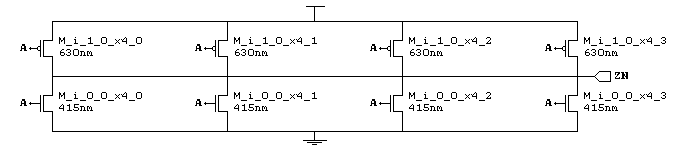
\includegraphics[width=1\linewidth]{../INV_X4/INV_X4.png}
	\caption{Reference schematic of the inverter}
	\label{fig:inv_png}
\end{figure}
\begin{figure}[H]
	\centering
	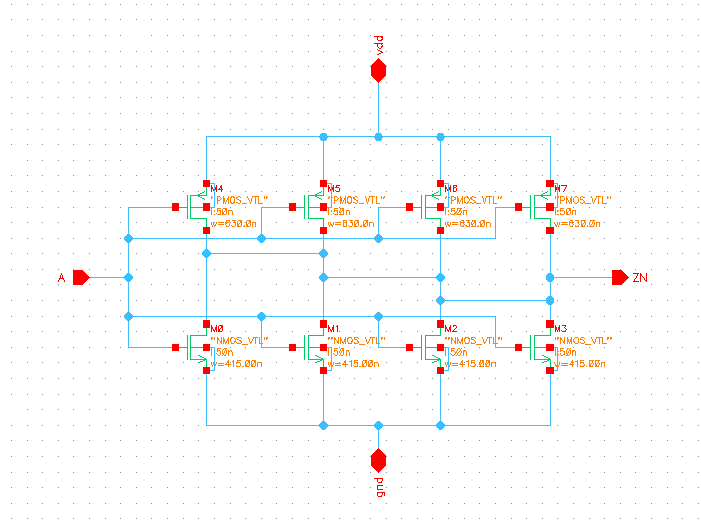
\includegraphics[width=\linewidth]{../INV_X4/INV_X4_schematic.png}
	\caption{Final schematic of \inv}
	\label{fig:inv_schematic}
\end{figure}

We then carried out some preliminary simulations using a test bench, to confirm that the circuit works correctly. We measured rise and fall times, as well as propagation delays, that will be compared with the actual characterization later on. We also measured the transfer characteristic, shown in figure \ref{fig:inv_tchar}.
\begin{figure}[H]
	\centering
	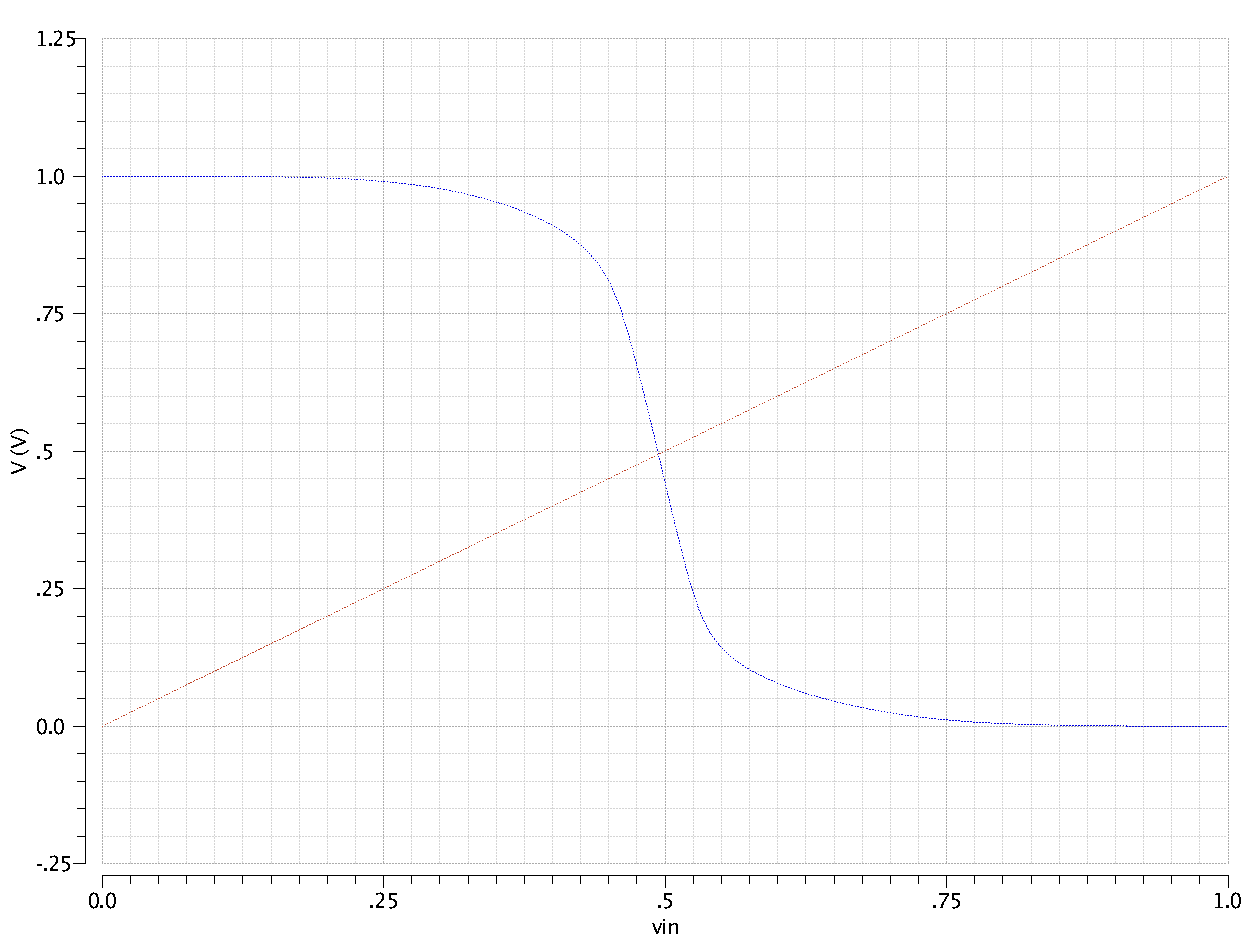
\includegraphics[width=.7\linewidth]{../INV_X4/INV_X4_transfer_char.pdf}
	\caption{Inverter transfer characteristic}
	\label{fig:inv_tchar}
\end{figure}

\subsection{Layout}
The final layout of \inv is shown in figure \ref{fig:inv_layout}. The main trick to note here is how we used transistor fingering extensively, by sharing as much as possible source and drain diffusions. This is generally done in order to reduce the total area of the standard cell, but in this case it was actually mandatory, because a single transistor large 4 times the minimum width would not fit inside the well height, at least for the PMOS pull-up network.
\begin{figure}[H]
	\centering
	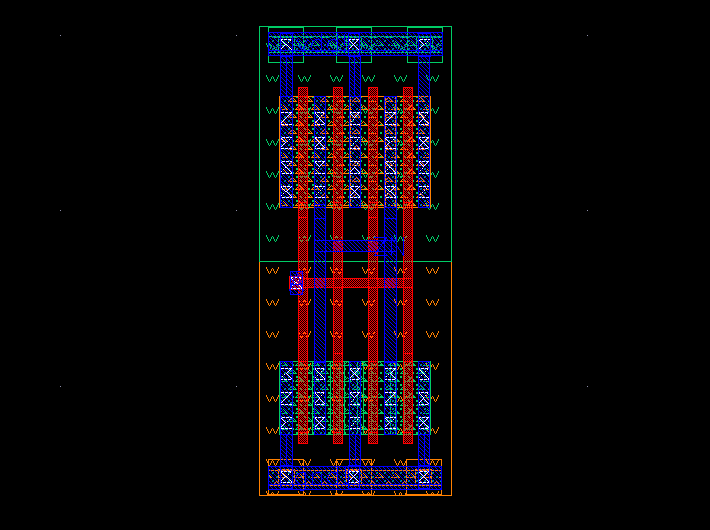
\includegraphics[width=\linewidth]{../INV_X4/INV_X4_layout.png}
	\caption{Layout of \inv}
	\label{fig:inv_layout}
\end{figure}

For PMOS transistors we were forced to finger four different transistor, while regarding the NMOS, probably, two fingered transistors with double width would have fit, but since the cell width would have been the same, we decided to go with four single width transistors anyway to improve symmetry.

Regarding pins, the output \texttt{ZN} did not cause any troubles and was placed on the rightmost metal strip connecting the drains of the PMOS and NMOS. As for the input \texttt{A}, instead, our first idea had been to place its via in the middle of the horizontal polysilicon strip, but then we noted that this way the external connections to that pin would have needed to cross the metal 1 layer, thus requiring metal 2 to be used instead. So eventually we settled with placing the via for the input on the leftmost part of the polysilicon, that does not force any metal 1 crossing and also more accurately reflects the topology of the schematic.

While developing the layout we ran the DRC tool many times to ensure all the design rules were met. After completing it we got the following final statement:
\newpage
\verbfilenobox[\small]{../INV_X4/INV_X4.drc.summary}
\newpage
Moreover, we compared layout and schematic netlists by using LVS, that succeeded on the first try with its reassuring smiling smiley-face:
\verbfilenobox[\small]{../INV_X4/INV_X4.lvs.report}

Just a note on the warning that says that nets \texttt{GND!} and \texttt{VDD!} are present in the layout but missing in the source (schematic). We tried to follow the steps of the laboratory sessions where the supply nets had the exclamation mark at the end in the layout view but not in the schematic one, and in fact we had no problems with this method for the \inv. However, we had a lot of issues for \ha when running LVS as it complained about missing power nets. We finally came to the conclusion that schematic and layout must have the exact same names for supply nets and that the exclamation mark can be avoided if the schematic does not exploit global nets to make the drawing cleaner and clearer. Even then, to this day it remains unclear why the inverter cell worked just as well with different names for power nets (disregarding this warning), while the half adder with the same setup caused so much trouble. We can only accept this and give in to the mighty secrets of Virtuoso.


\subsection{Characterization}
\label{sec: inv_char}
The first step toward the complete characterization of our logic gate was the extraction of the parasitic elements from the layout. To do this, we ran the PEX tool from the layout editor and got the following report as well as a complete new netlist that takes into account those parasitics in the schematic.
\verbfilenobox[\small]{../INV_X4/INV_X4.pex.report}

Then, we generated a new config view for our cell and linked it to the calibre view, which contains the aforementioned netlist with the parasitics. We then set up the old test bench to use this new view and ran the automatic simulations needed to compile the Liberty file and compare with the schematic simulations.

In order to fill in the Liberty file faster we developed a Matlab script that convert the traces exported in \texttt{.csv} from Virtuoso into the correct format for the \texttt{.lib} file, which is shown in the following snippet:
\verbfilenobox[\small]{../INV_X4/INV_X4.lib}

We also developed another Matlab script to plot the results of the simulations, shown in the following figures.
\begin{figure}[H]
	\centering
	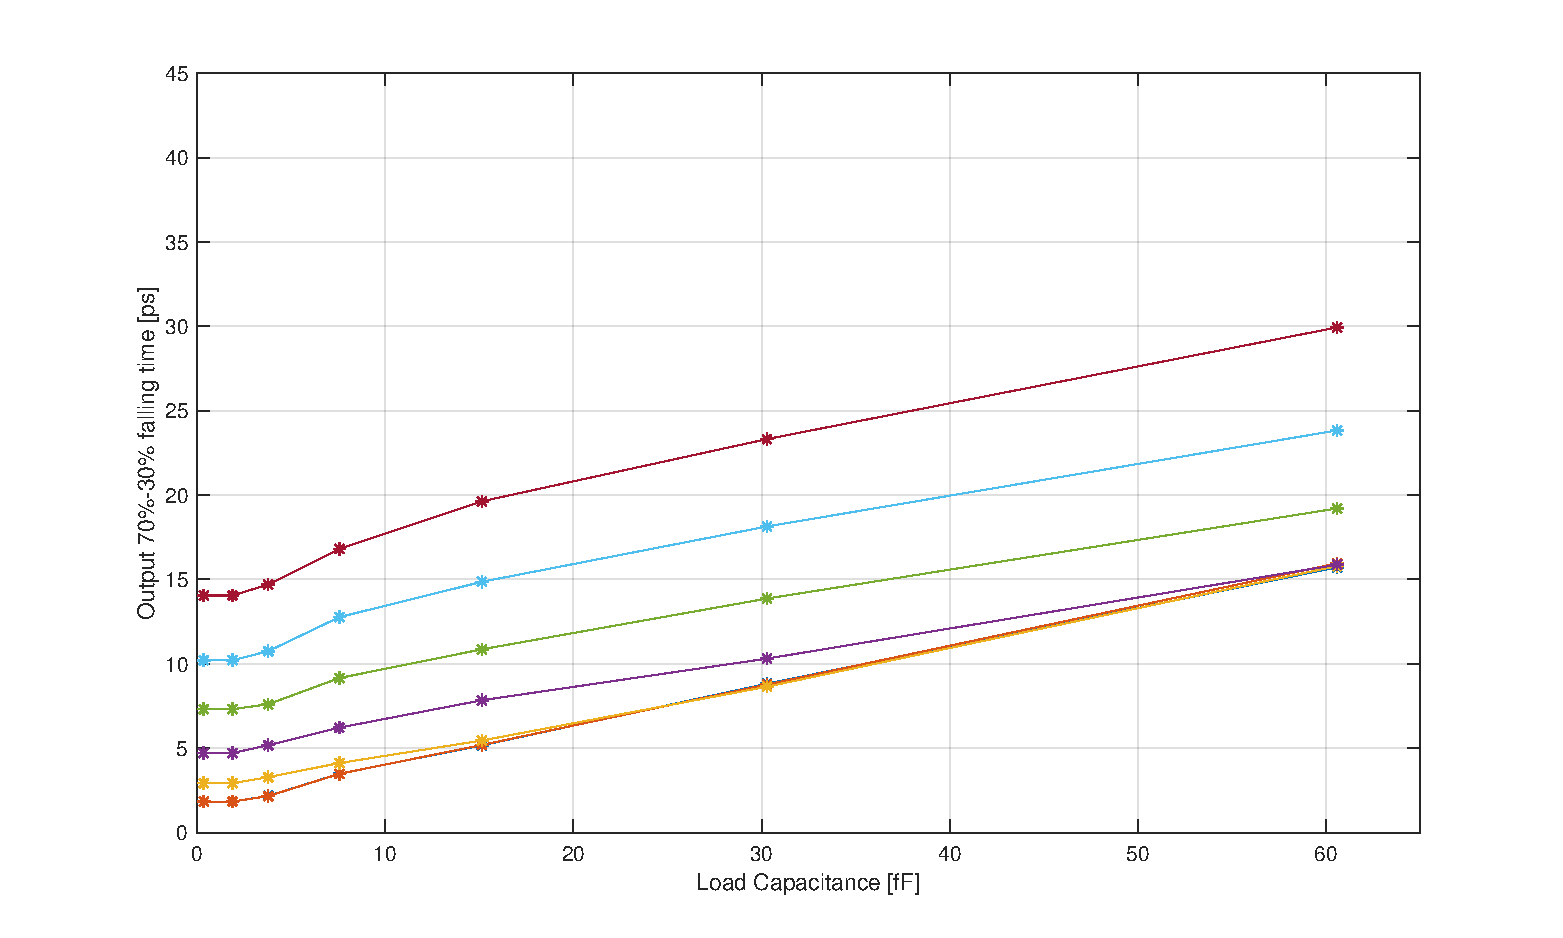
\includegraphics[width=\linewidth]{../INV_X4/simulations/t_F.pdf}
	\caption{Fall time vs load capacitance, higher curves are for longer input rise times.}
	\label{fig:inv_t_F}
\end{figure}
\begin{figure}[H]
	\centering
	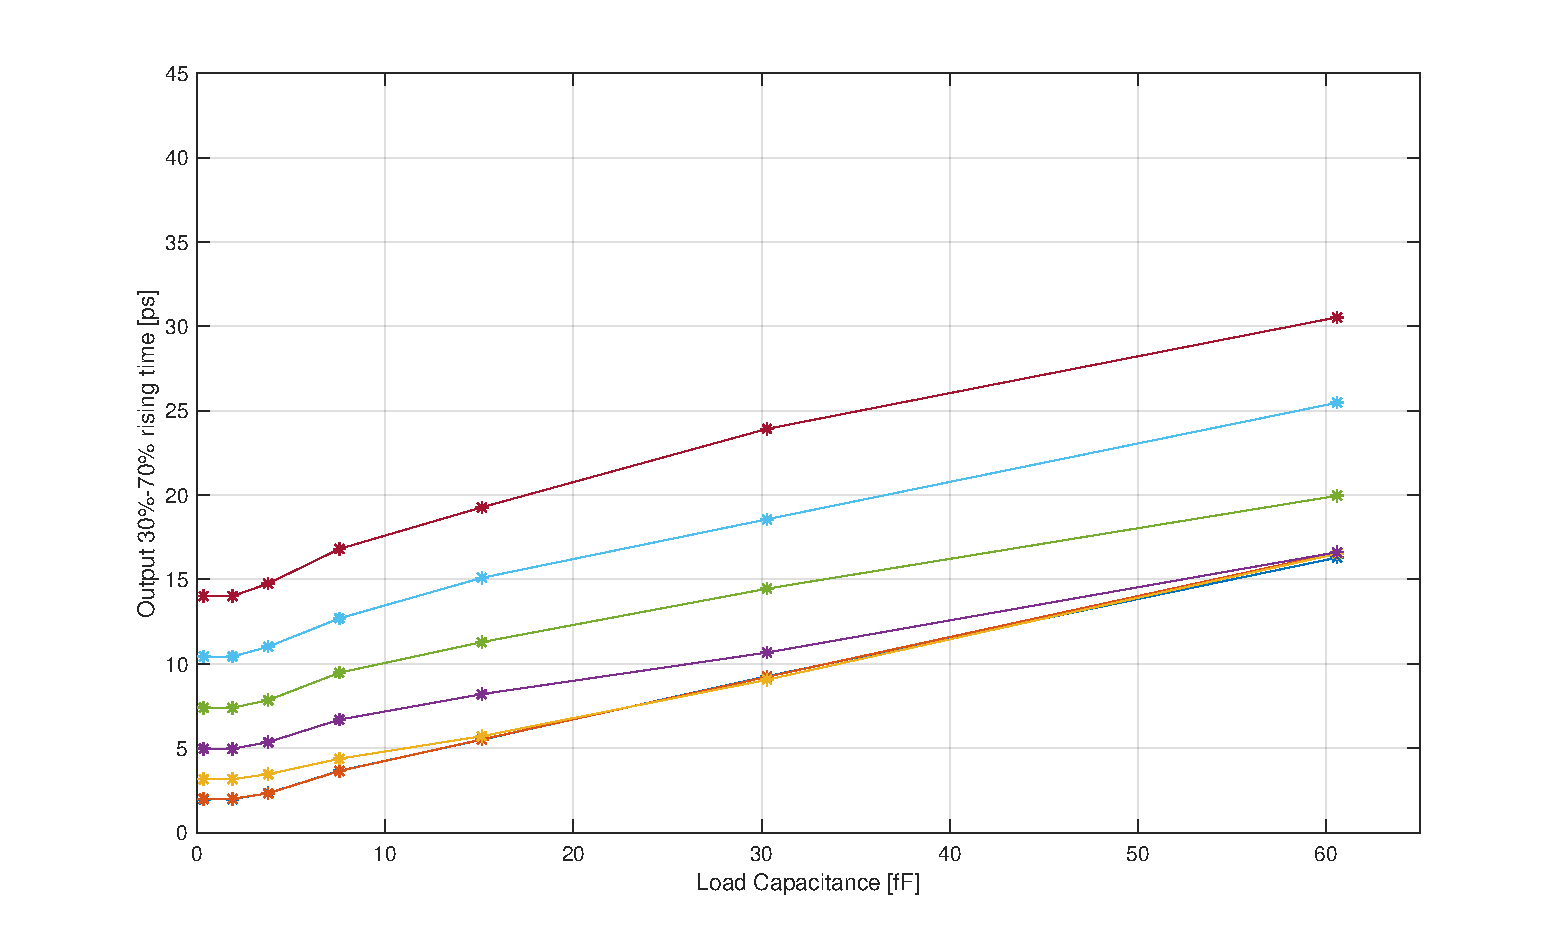
\includegraphics[width=\linewidth]{../INV_X4/simulations/t_R.pdf}
	\caption{Rise time vs load capacitance, higher curves are for longer input fall times.}
	\label{fig:inv_t_R}
\end{figure}
\begin{figure}[H]
	\centering
	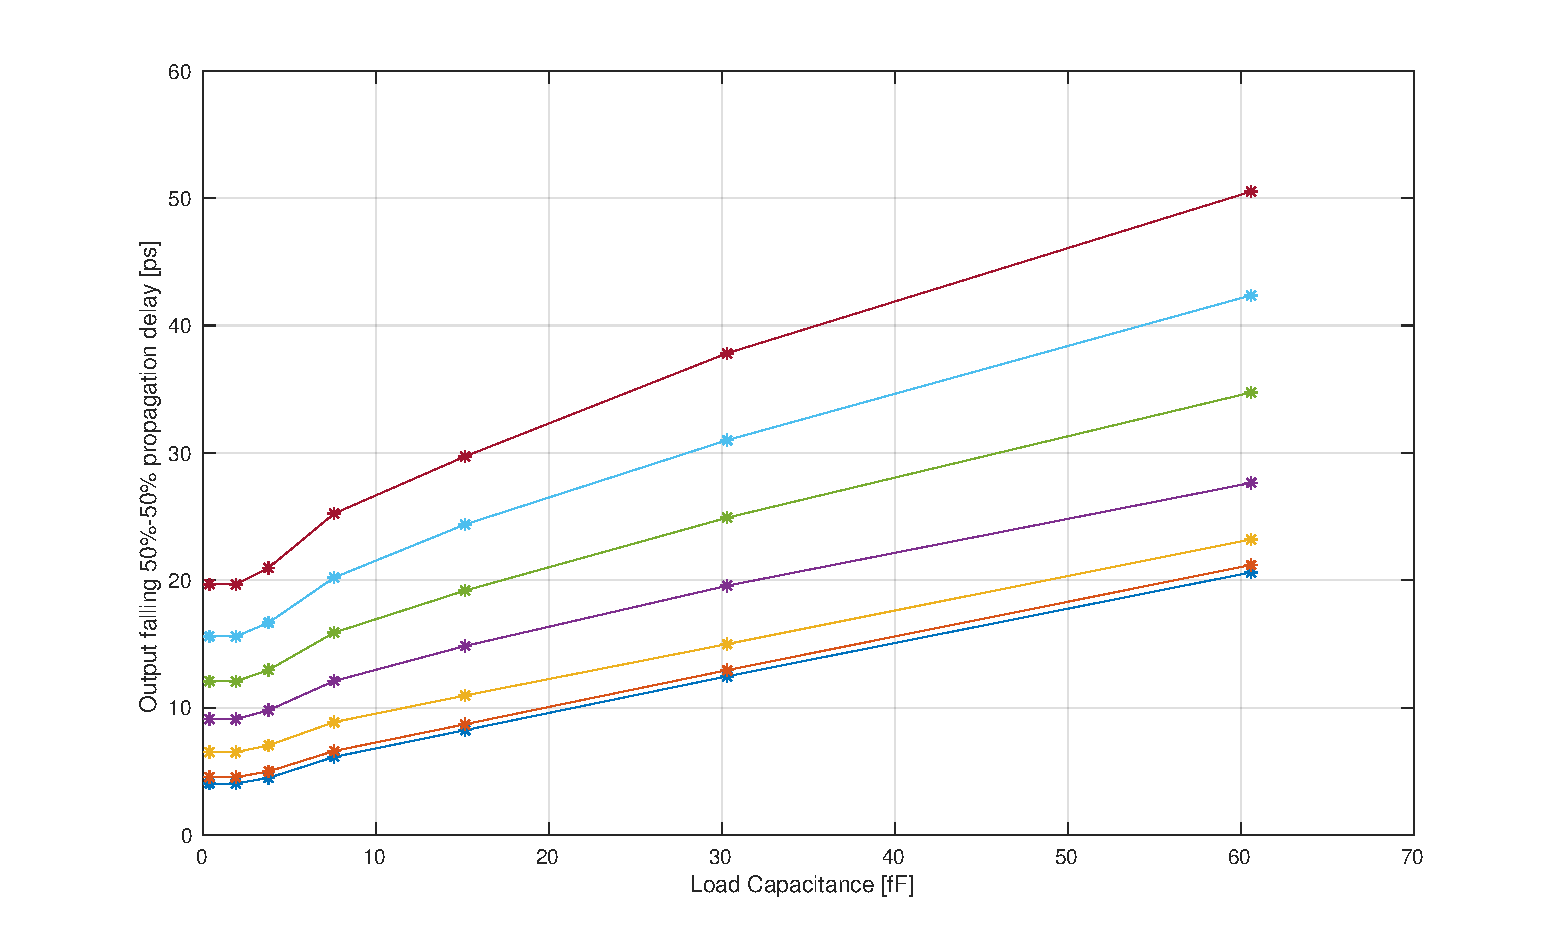
\includegraphics[width=\linewidth]{../INV_X4/simulations/tp_L.pdf}
	\caption{Falling propagation delay vs load capacitance, higher curves are for longer input rise times.}
	\label{fig:inv_tp_L}
\end{figure}
\begin{figure}[H]
	\centering
	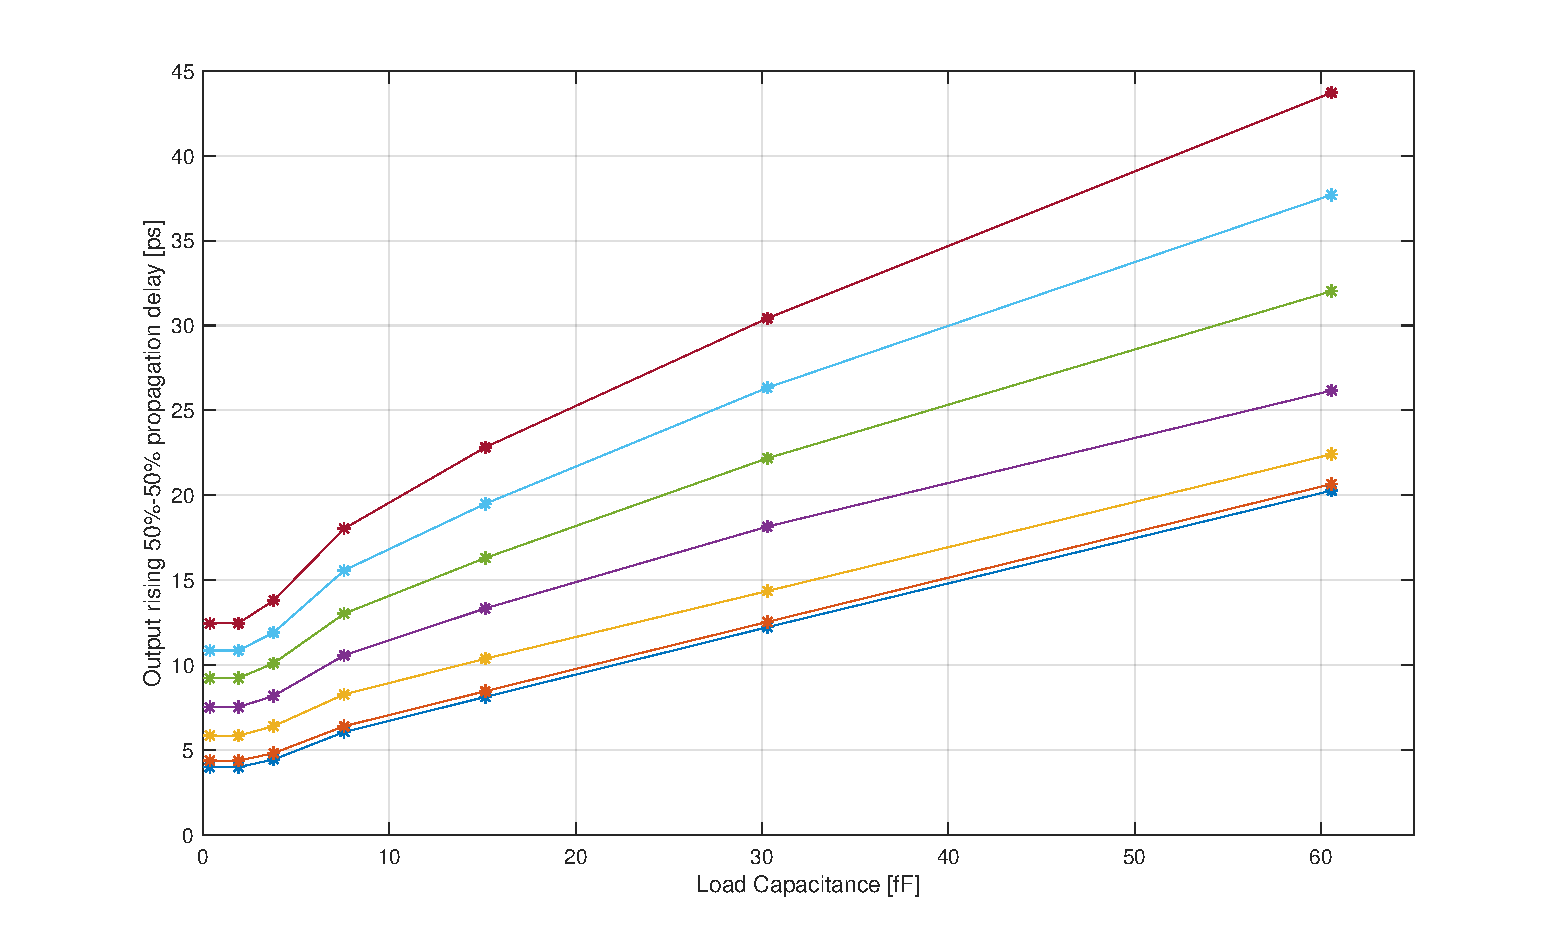
\includegraphics[width=\linewidth]{../INV_X4/simulations/tp_H.pdf}
	\caption{Rising propagation delay vs load capacitance, higher curves are for longer input fall times.}
	\label{fig:inv_tp_H}
\end{figure}

We also compared these results with the simulation done on the original schematic, computing the relative difference in the measured parameters for a given input delay (different input delay values gave similar results and thus were not meaningful to show).
\begin{figure}[H]
	\centering
	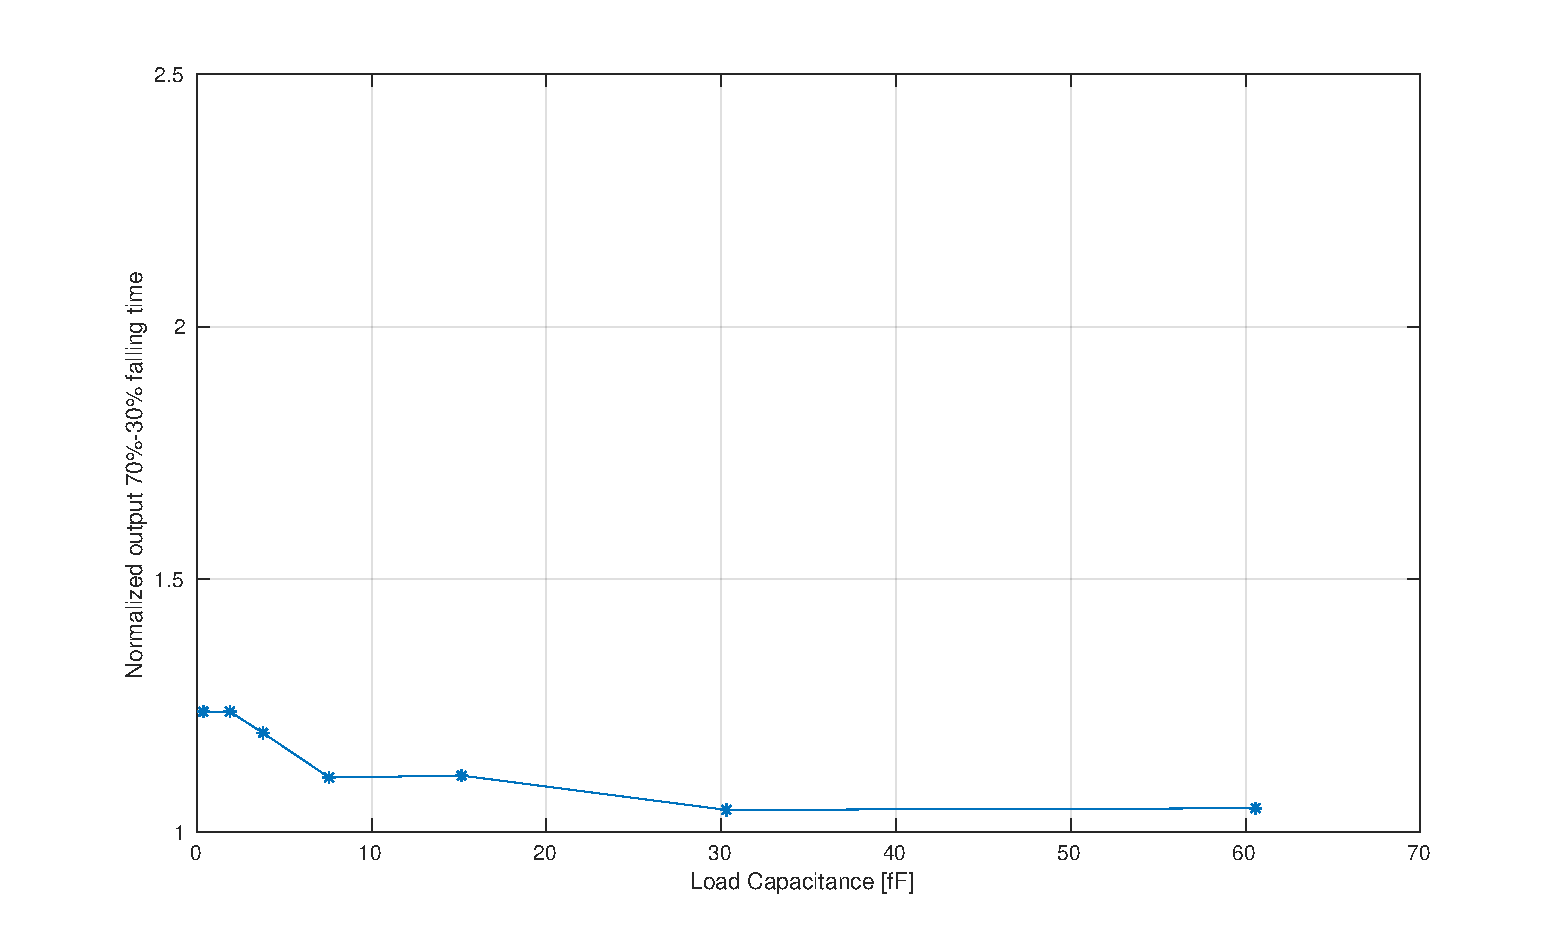
\includegraphics[width=\linewidth]{../INV_X4/simulations/t_F_diff.pdf}
	\caption{Relative fall time difference vs load capacitance}
	\label{fig:inv_t_F_diff}
\end{figure}
\begin{figure}[H]
	\centering
	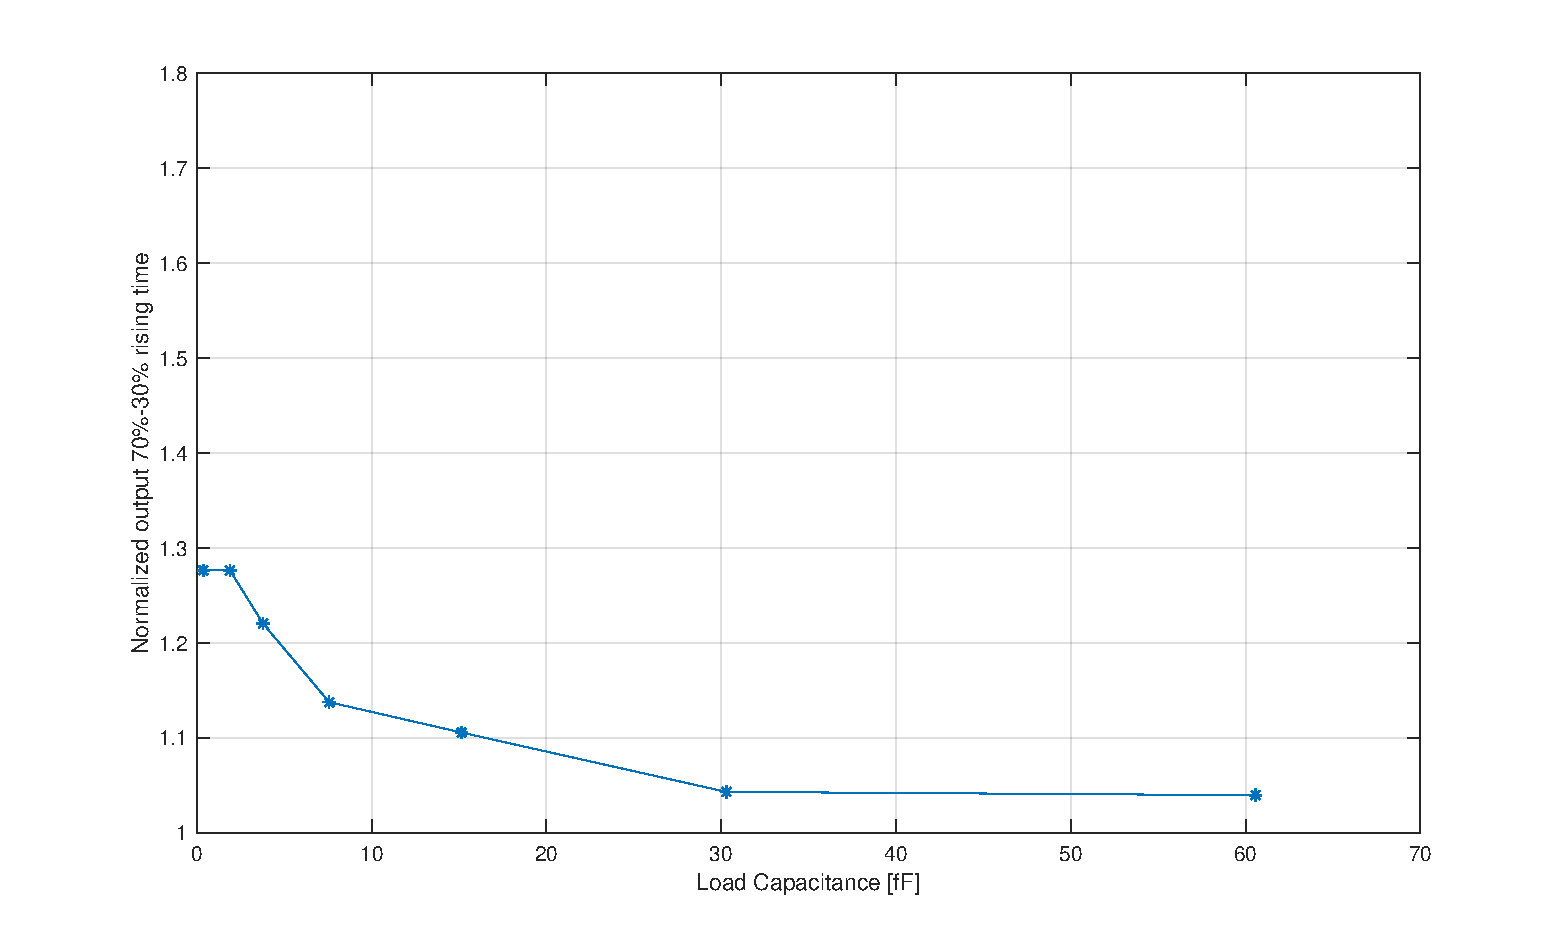
\includegraphics[width=\linewidth]{../INV_X4/simulations/t_R_diff.pdf}
	\caption{Relative rise time difference vs load capacitance}
	\label{fig:inv_t_R_diff}
\end{figure}
\begin{figure}[H]
	\centering
	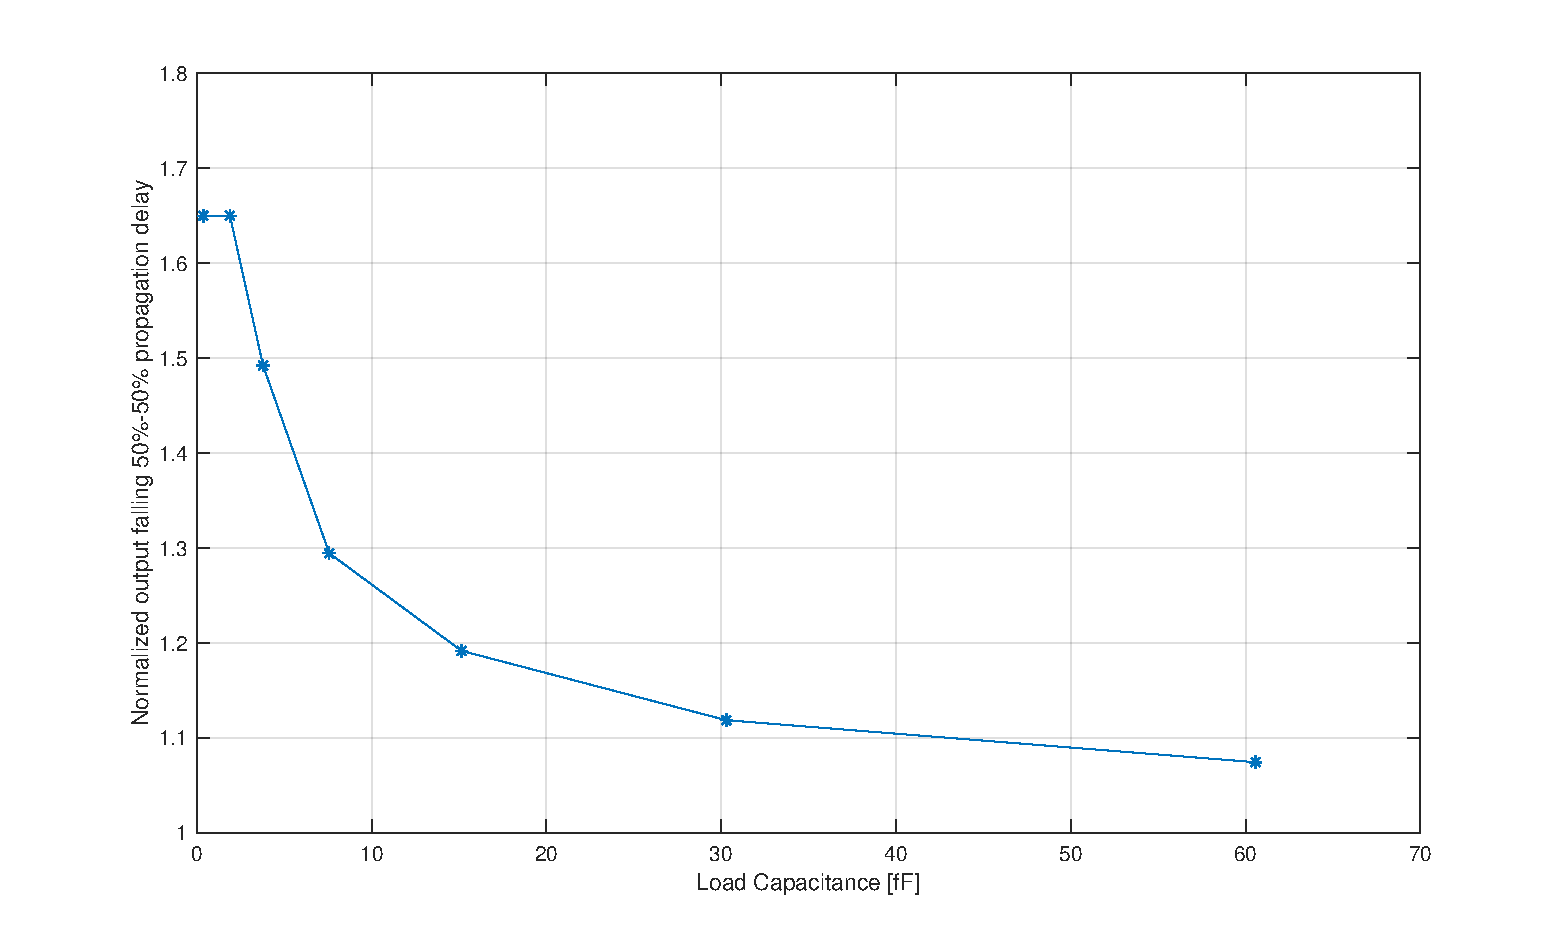
\includegraphics[width=\linewidth]{../INV_X4/simulations/tp_L_diff.pdf}
	\caption{Relative falling propagation delay difference vs load capacitance}
	\label{fig:inv_tp_L_diff}
\end{figure}
\begin{figure}[H]
	\centering
	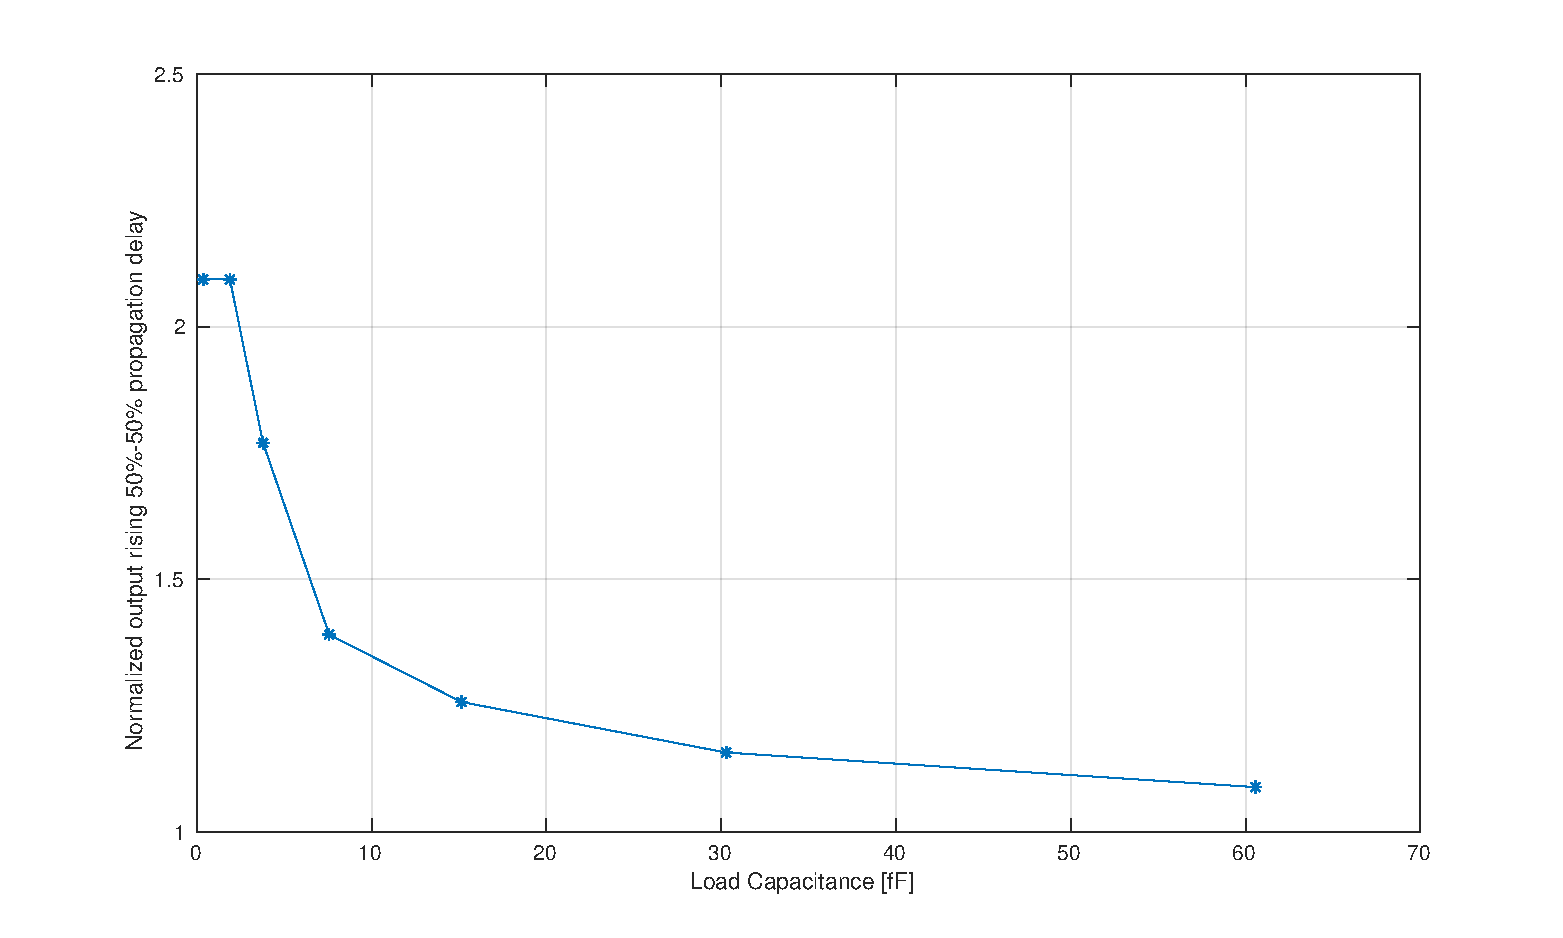
\includegraphics[width=\linewidth]{../INV_X4/simulations/tp_H_diff.pdf}
	\caption{Relative rising propagation delay difference vs load capacitance}
	\label{fig:inv_tp_H_diff}
\end{figure}

We can note that for very small load capacitance values the simulations done on the extracted parasitics show steadily longer delays, from 20\% to 45\% longer than the schematic-only simulations. This is easily explained by the fact that the parasitic elements have a bigger impact on performance when the load capacitance is very small, while for large values of load capacitance its effect becomes dominant and the weight of the parasitic contributions drastically reduces.

The case of the rising propagation delay is a bit different in that it shows a very large difference between simulations for small load capacitance values: greater that 100\%. This behavior has shown to be consistent among different measurements and tests, but we could not really explain why it shows up, as we expected rising and falling delays to be more or less symmetrical.

\section{Half adder}
\subsection{Schematic}
<<<<<<< HEAD
The schematic was drawn using Virtuoso Schematic Editor (figure \ref{fig: HAX1_sch}), following the reference \texttt{.png} shown in figure \ref{fig: HAX1_png}.

\begin{figure}[H]
	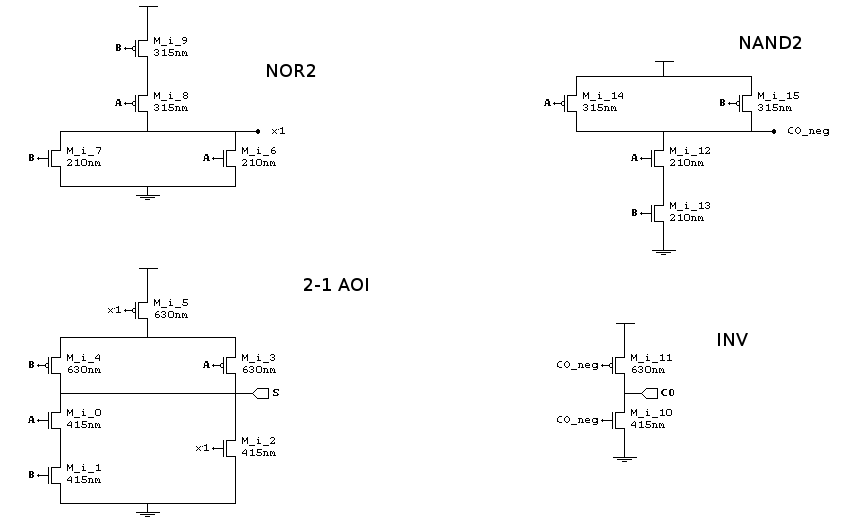
\includegraphics[width=0.9\linewidth]{./Images/HA/HA_X1.png}
	\caption{Reference schematic of the half-adder}
	\label{fig: HAX1_png}
\end{figure}
=======
The schematic was drawn using Virtuoso schematic editor. We used the following .png file as reference.

\begin{figure}[H]
      \centering
       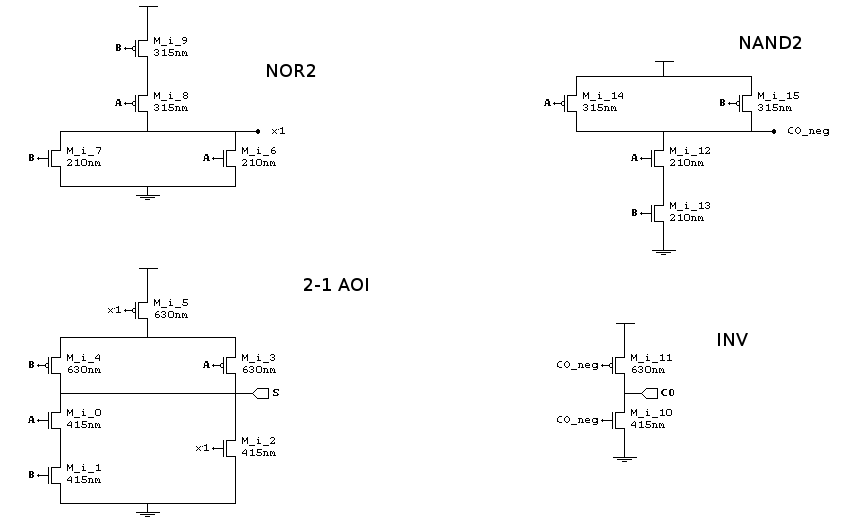
\includegraphics[width=12cm]{./Images/HA/HA_X1.png}
\caption{HAX1 schematic-source}
\label{fig: HAX1_sch_sc}
\end{figure}

Even though the 2-1 AOI has the pull up net with a series pMos connected through the power supply and two pMos in parallel, we decided to switch the two subnets to obtain better perfomances. There are two main reasons for this choice:
\begin{enumerate}
\item If A and B are both at '0' and x1 is at '1', the intermediate node is discharged. When a transition of x1 happens then the node has to be charged from only one $R_{eq}$. With two pMos between the supply and the other transistor the situation could be hypotetically better: in the worst case we could have the same situation as before, but if both A and B are asserted then the capacitance takes less time to complete the charging.  
\item The capacitance of the intermidiate node is greater if there are 2 pMos before the output instead of one.
\end{enumerate}

We report here the final schematic used to create the layout.
>>>>>>> f7faa04fc7b7c1117da879bf7a5786b0138803b3

\begin{figure}[H]
      \centering
       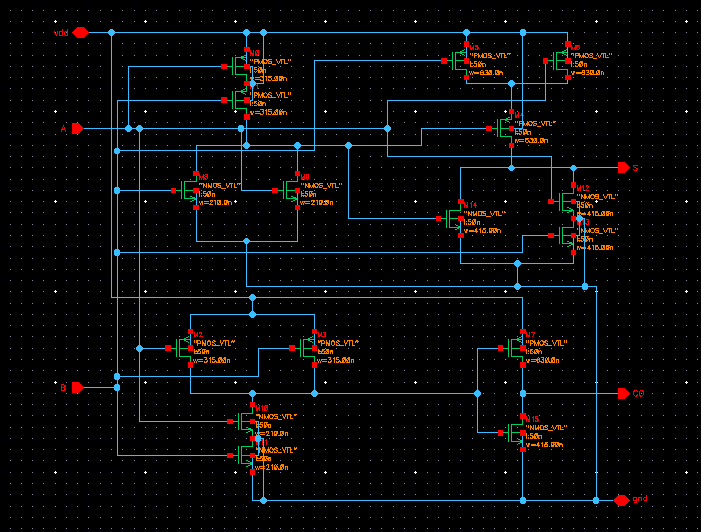
\includegraphics[width=\linewidth]{./Images/HA/HAX1_schematic.png}
\caption{HAX1 schematic}
\label{fig: HAX1_sch}
\end{figure}

We created a testbench and simulated the circuit as we did for the inverter. Everything was correct.

\begin{figure}[H]
      \centering
       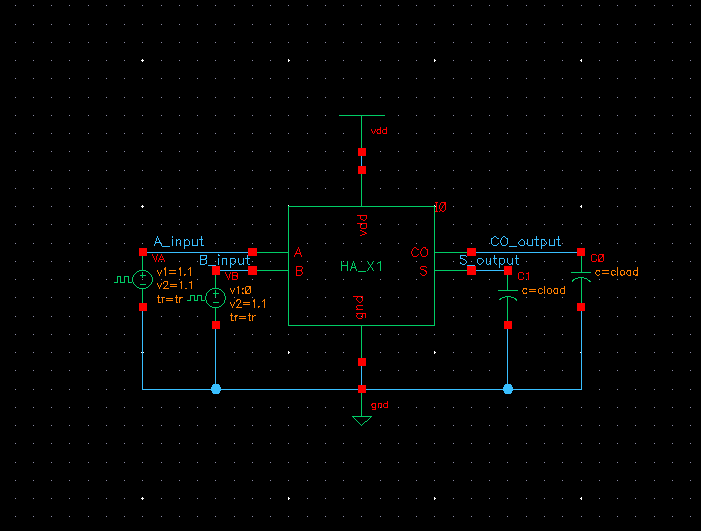
\includegraphics[width=12cm]{./Images/HA/HAX1_TB_schematic.png}
\caption{HAX1 testbench}
\label{fig: HAX1_tb}
\end{figure}

\subsection{Layout}
Given that the layout of the half adder is quite more complex than the one of the inverter, we started by deeply analyzing the possible approaches using the pen-and-paper method. The final solution that we found consisted in sharing source/drain diffusions as much as possible, in order to minimize the area in the horizontal direction, similarly to what we did in the inverter design.

When actually drawing the design in Virtuoso, we made sure of running the Design Rule Checker (DRC) very often, in order to avoid problems in advance. The final result of this tool is totally similar to the one we obtained for the \inv in section \ref{sec: inv_sch}, and thus omitted.

Layout design started looking at the schematic. First of all we tried to put the two outputs on the opposite sides of the cell, because this way, if the input are brought over it in the middle with the \texttt{metal 2} and linked with vias, the input-output paths are more probably balanced in lenght, keeping the input polysilicon lines shorter and therefore reducing these lines' propagation delays. This assumption lead us to place the carry-out generation network (a NAND gate followed by an inverter) on the left of the layout, and the sum generation network (NOR gate followed by an AOI12 gate) on the righ side.
Thus we started drawing on a paper the first NMOS of the inverter whose output was CO. With a view to share the sources/drains as much as possible we began putting all the transistors one near the other drawing only the strictly necessary metal.
We used different colours to have an easier readability and go on drawing only the \texttt{metal} for the sources/drains and the \texttt{polysilicon} for the gates until the end of the port and left the routing at last. Then we completed the layout linking together the various elements coherently with the schematic view. The resulting pencil draw is reported in figure \ref{fig: lay_drw}.

\begin{figure}[H]
      \centering
      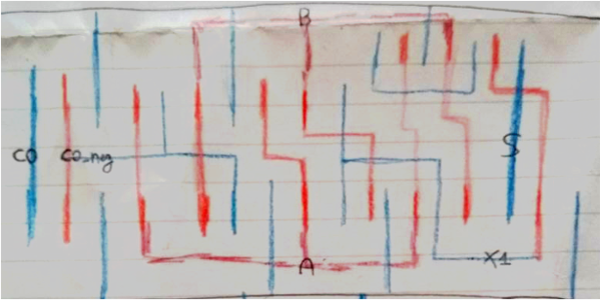
\includegraphics[width=0.8\linewidth]{./Images/HA/layout_drw.png}
	  \caption{First sketch of the layout. \textcolor{blue}{Blue}: metal1, \textcolor{red}{red}: polysilicon. Labels do not match the position of the corresponding vias.}
	  \label{fig: lay_drw}
\end{figure}

Then we converted this sketch in a real layout design using the Virtuoso embedded layout editor. During our sessions we paid attention to reduce every distance to the minimum with the aid of the meter tool and in accordance with the Design Rules. We made a lot of effort to have a cell with the minimum area because the area is directly linked to the yield of the process and to logic ports density, capacitance and therefore delay and power cost per commutation. The less is the area, the more ports can stay in a chip or the more the chip will be small, and it is harder to find defects on a single chip if it is small, because the density of the defects per unit area is about constant (higher yield for the process). The delay and the power costs rise with the area because if more material is used, more resistance/capacitance is added. For this reason we also tried to reduce the length of every wire.

The height of the cell is fixed because of the standard-cell format requirements. Its top and ground lines, whose purpose id to feed the transistors, are made of \texttt{metal1}. Many entity like this one can be put one next to the other to form a row of cells packed together and fed with global $V_{DD}$ and $GND$ voltage lines.

When we drew the layout with the editor we changed a little bit the connections. Instead of putting a single wire of \texttt{polysilicon} to connect each gate with the related input A/B, we used vias and \texttt{metal1} pieces of line. It would have been interesting to compare the performances of two implementations, to see whether longer polysilicon lines permorm better or worse than sorter ones connected through metal lines and vias. Both the layouts are reported in figure \ref{fig: HAX1_layouts}, though only the polysilicon and metal version (figure \ref{fig: polymetal}) has been simulated and characterized due to the lack of time.

\begin{figure}[H]
    \centering
    \begin{subfigure}[h]{0.8\textwidth}
        \centering
        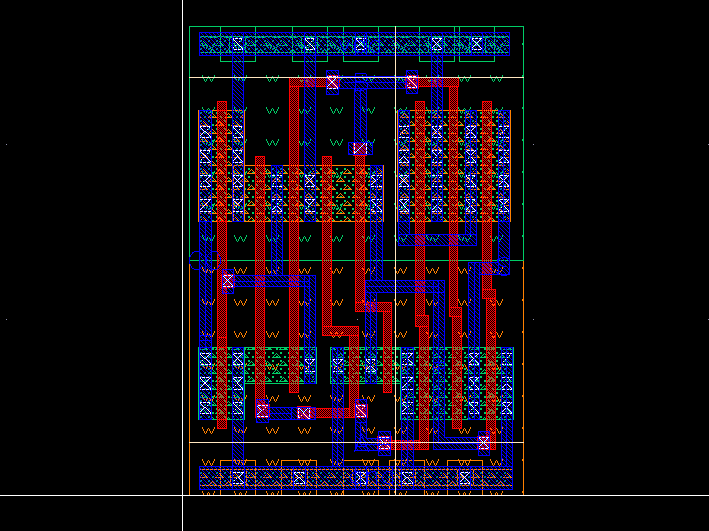
\includegraphics[width=\linewidth]{./Images/HA/HAX1_poly-metal_layout.png}
        \caption{Polysilicon and metal input lines}
		\label{fig: polymetal}
    \end{subfigure}
    \begin{subfigure}[b]{0.8\textwidth}
        \centering
        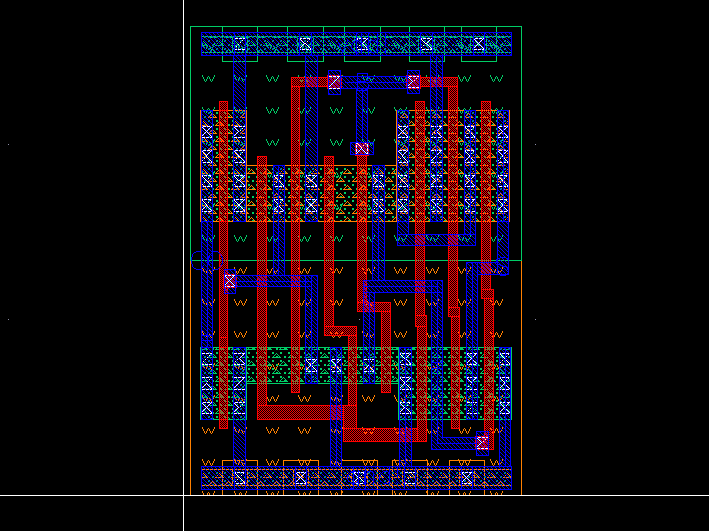
\includegraphics[width=\linewidth]{./Images/HA/HAX1_poly_layout.png}
        \caption{Polysilicon only input lines}
		\label{fig:poly}
    \end{subfigure}
    \caption{Different layouts}
    \label{fig: HAX1_layouts}
\end{figure}

Notice how the final layout in figure \ref{fig: polymetal} appears divided in two different active region both for the NMOS and PMOS networks. This is necessary whenever two metal lines are connected to the active region without a gate between them. In fact, during the manufacturing process, the polysilicon layer is lay before the active one. Therefore, the gates prevent the active regions to extend below them, even if the layout masks do. This automatically isolates the drain and source implants and the related metal lines. When no gate is lay between two metal lines, the isolation must be considered as part of the active layer mask. In the early stages of the development this wasn't clear to us, as proved by figure \ref{fig:poly}.

Finally we launched the LVS and then extracted the parasitic elements. The PEX operation gave us a schematic with all the MOS with the relative parasitics. The net is implicit because no wire is drawn, but every terminal has its own reference. The following figures show the group of the 16 MOS of the cell, a detail of one MOS to highlight the labels on the terminals and a parasitic capacitance between the drain of that MOS and gnd. 

\begin{figure}[H]
      \centering
       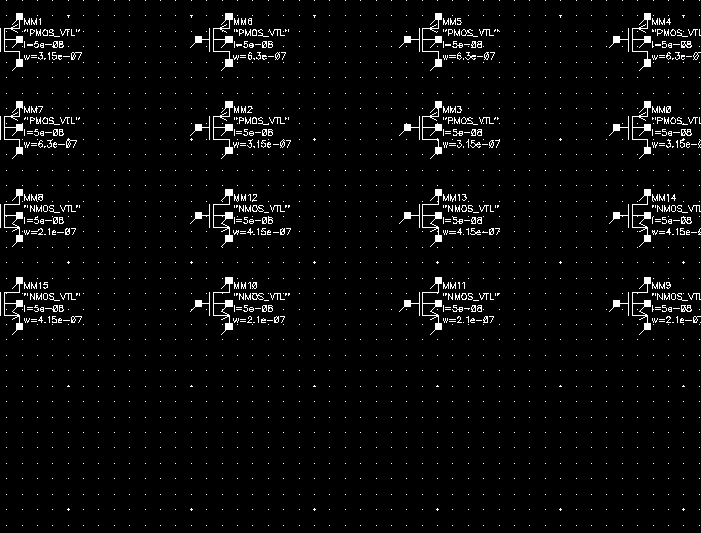
\includegraphics[width=12cm]{./Images/HA/HAX1_PEX.png}
\caption{Detail of the extracted parasitics - group of MOS}
\label{fig: PEX0}
\end{figure}

\begin{figure}[H]
      \centering
       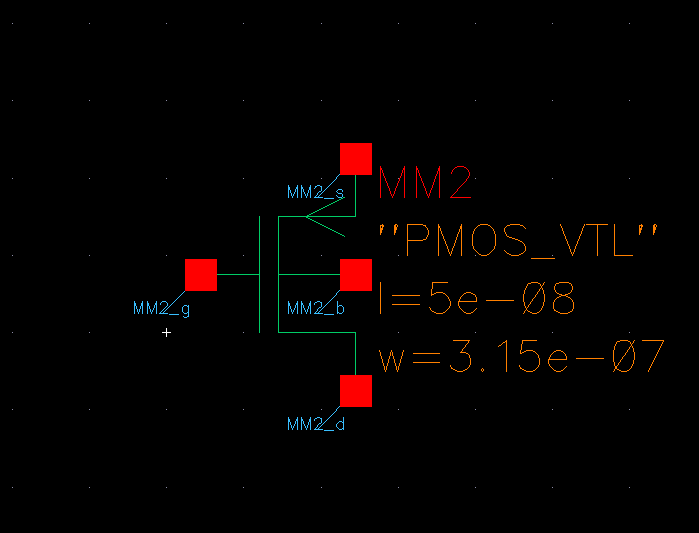
\includegraphics[width=12cm]{./Images/HA/HAX1_PEX_1.png}
\caption{Detail of the extracted parasitics - MOS M2}
\label{fig: PEX1}
\end{figure}

\begin{figure}[H]
      \centering
       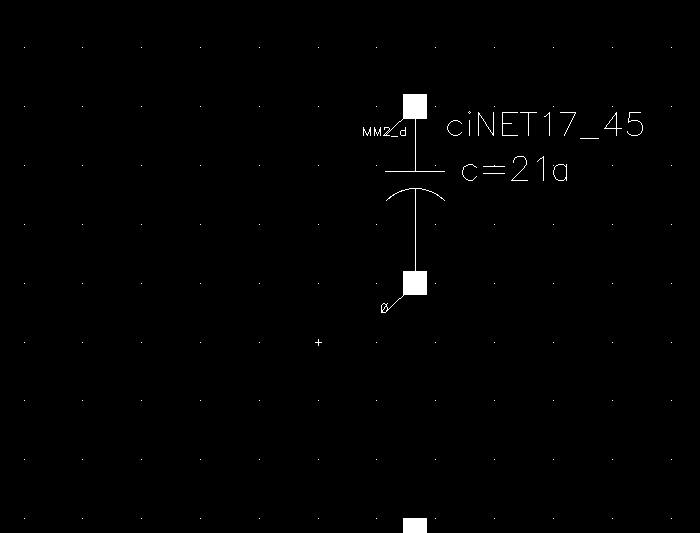
\includegraphics[width=12cm]{./Images/HA/HAX1_PEX_2.png}
\caption{One parasitic capacitance, between the drain of M2 and gnd}
\label{fig: PEX2}
\end{figure}

Every reference can be spotted looking at the schematic and at the relative file. The PEX produced also the report and the netlist files. In the netlist all the informations about the net with the parasitics can be found. For example here we report the part related with the previous pictures.

\begin{figure}[H]
      \centering
       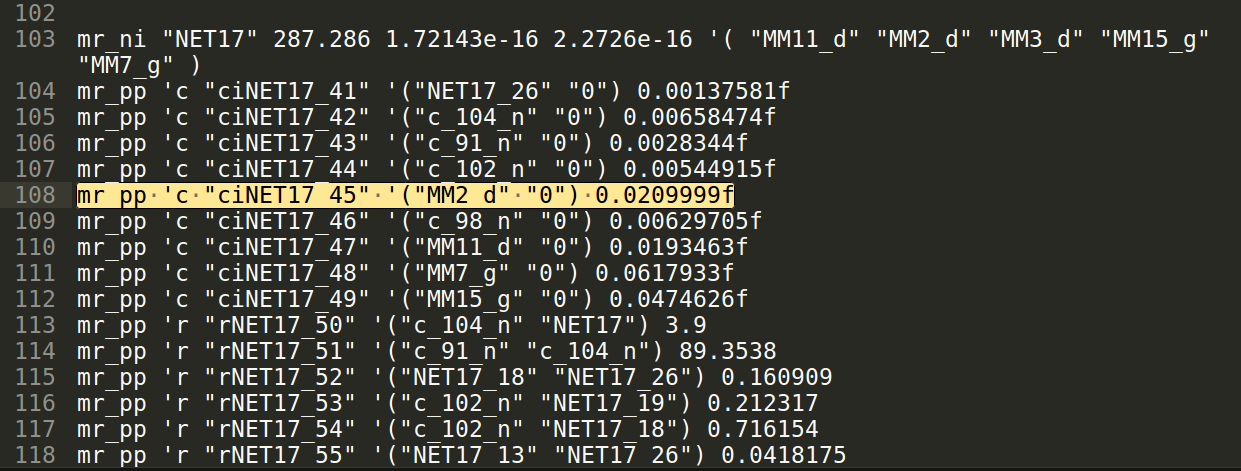
\includegraphics[width=12cm]{./Images/HA/HAX1_PEX_netlist.png}
\caption{Part of the file 'HA-X1.pex.netlist'}
\label{fig: PEX0_netlist}
\end{figure}


\subsection{Characterization}
As done before, we proceeded with the lumped parameters extraction from the designed layout using the PEX tool. Again, the output log and schematic listed all the extracted resistances and capacitances similarly to what has been reported for the \inv in section \ref{sec: inv_char}. From the extracted data we created a new cell configuration (\texttt{config} view) for the \ha. At this point we created a new testbench cell, where we imported our \ha as DUT. Two pulse generators and two load capacitors with parametric values completed the testbench along with the $V_{DD}$ and $GND$ ports.

At this point we were ready to perform the simulations required to fill the timing characterization tables in the Liberty file.
\begin{itemize}
	\item \textbf{Carry-out} Since the \texttt{CO} generation network is an \texttt{AND} gate of the two inputs \texttt{A} and \texttt{B}, it is necessary to have one of these inputs to be fixed at its high value for the output to switch. Therefore only eight measurements are required to fully characterize this output pin: output falling and rising propagation delays, output fall and rise time, each of these related to both \texttt{A} and \texttt{B} inputs.

	\item \textbf{Sum} The \texttt{S} generation network is a \texttt{XOR} gate. Its output can thus switch whenever the inputs change from being equal to being different and viceversa. Therefore sixteen measurements are required. It is important to notice that unlike \texttt{CO}, this output shows an inverting behaviour with respect to the related input when the other input is high.
\end{itemize}

Having set properly the measurement parameters in the ADE L simulation environment we ran the parametric simulation with the same input transition times and load capacitance values used for the \inv. 


\end{document}
